\documentclass[tikz,border=10pt]{standalone}
\usepackage{tikz}
\usepackage{amsmath}
\usepackage{amsfonts}
\usetikzlibrary{arrows.meta,positioning,shapes.geometric,shapes.misc,fit,backgrounds,calc,decorations.pathreplacing,patterns}

% Define colors used in the comprehensive report
\definecolor{cwBorder}{RGB}{128,128,128}
\definecolor{cwFlow}{RGB}{70,130,180}
\definecolor{cwAlert}{RGB}{220,20,60}
\definecolor{cwDecoy}{RGB}{255,140,0}

\begin{document}
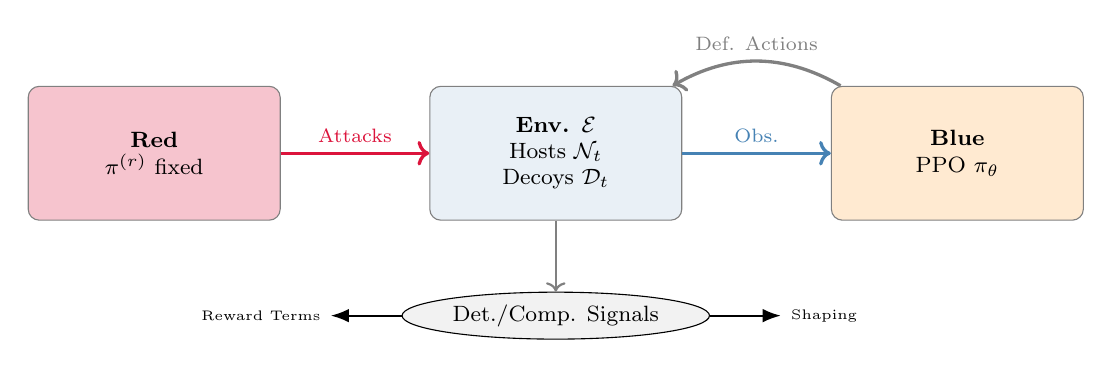
\begin{tikzpicture}[font=\footnotesize,node distance=1.9cm,sys/.style={draw=cwBorder,rounded corners,minimum width=3.2cm,minimum height=1.7cm,align=center,fill=white}]
    % Nodes tightened
    \node[sys,fill=cwAlert!25] at (0,0) (red) {\textbf{Red}\\$\pi^{(r)}$ fixed};
    \node[sys,fill=cwFlow!12] at (5.1,0) (envInt) {\textbf{Env. $\mathcal{E}$}\\Hosts $\mathcal{N}_t$\\Decoys $\mathcal{D}_t$};
    \node[sys,fill=cwDecoy!18] at (10.2,0) (blue) {\textbf{Blue}\\PPO $\pi_\theta$};
    % Arrows
    \draw[->,very thick,cwAlert] (red) -- node[above,font=\scriptsize]{Attacks} (envInt);
    \draw[->,very thick,cwFlow] (envInt) -- node[above,font=\scriptsize]{Obs.} (blue);
    \draw[->,very thick,cwBorder] (blue) to[out=150,in=30] node[above,font=\scriptsize]{Def. Actions} (envInt);
    % Signals ellipse condensed
    \node[draw,ellipse,fill=cwBorder!10,inner sep=2pt,below=0.9cm of envInt] (signals) {Det./Comp. Signals};
    \draw[->,thick,cwBorder] (envInt) -- (signals);
    \draw[-Latex,thick] (signals.west) -- +( -0.9,0) node[left,font=\tiny]{Reward Terms};
    \draw[-Latex,thick] (signals.east) -- +( 0.9,0) node[right,font=\tiny]{Shaping};
\end{tikzpicture}
\end{document}